\newpage
\appendix

\chapter{Example of deploying an IOC with YAML file}
An example yaml file used to deploy \gls{IOC}. In this particular case, the IOC was operating a BINDER MK240 climatic chamber using Modbus protocol. The volumes are used to acquire database files and also synchronize the time with the node. Moreover, the container run in the host network and the so-called pseudo terminal is activated (tty). 
\label{YAML}
\begin{verbatim}

version: "3.7"
services:
  binder:
    container_name: binderioc
    volumes:
      - "/home/cbm/dcs-sts/config/:/config"
      - "/etc/localtime:/etc/localtime:ro"
      - "/etc/timezone:/etc/timezone:ro"
    network_mode: "host"
    image: "paluma.rub.de/panda-ioc"
    tty: true
    command: /config/iocBoot/iocBinder/st.cmd
\end{verbatim}

\chapter{CSA scans for modules of the mSTS}
\label{CSA}
The plots presented below show the behavior of the not-presented modules during the data-taking and operation of the mSTS. 

\begin{figure}[h!]
\centering
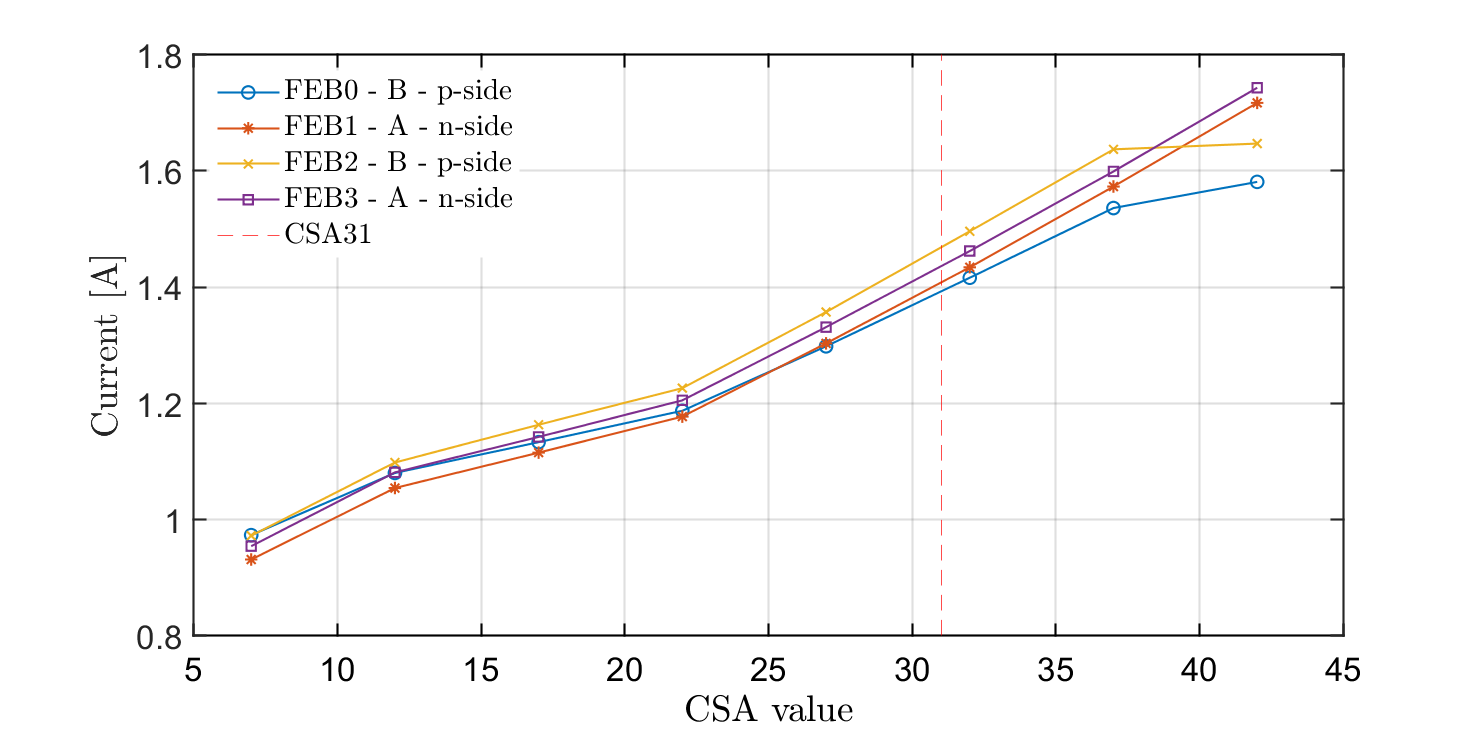
\includegraphics[width=0.9\columnwidth]{Chapter6/DCS/images/U1CSABIAS.png}
\caption{CSA scan of the unit 1}
\label{U1CSABIAS}
\end{figure}

\begin{figure}[h!]
\centering
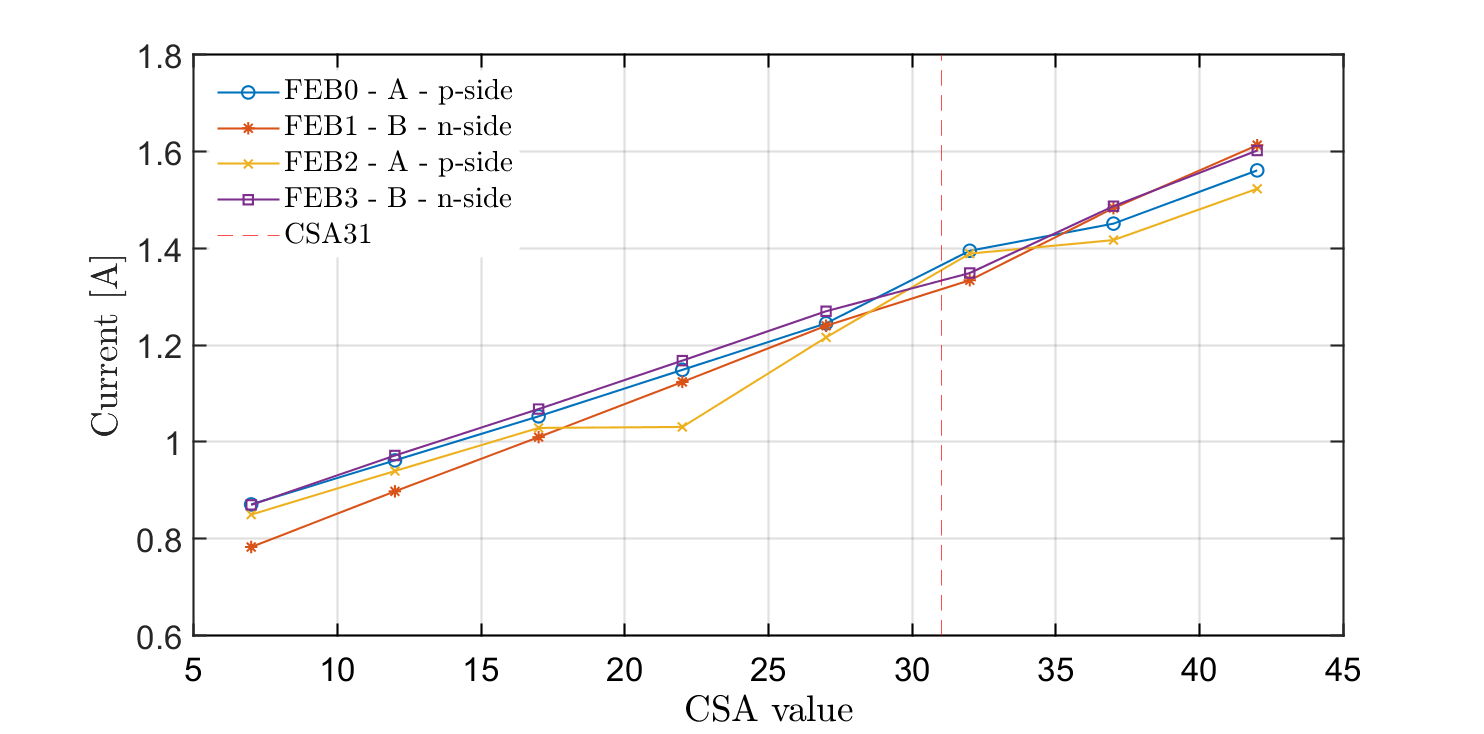
\includegraphics[width=0.9\columnwidth]{Chapter6/DCS/images/U2CSABIAS.png}
\caption{CSA scan of the unit 2}
\label{U2CSABIAS}
\end{figure}

\begin{figure}[h!]
\centering
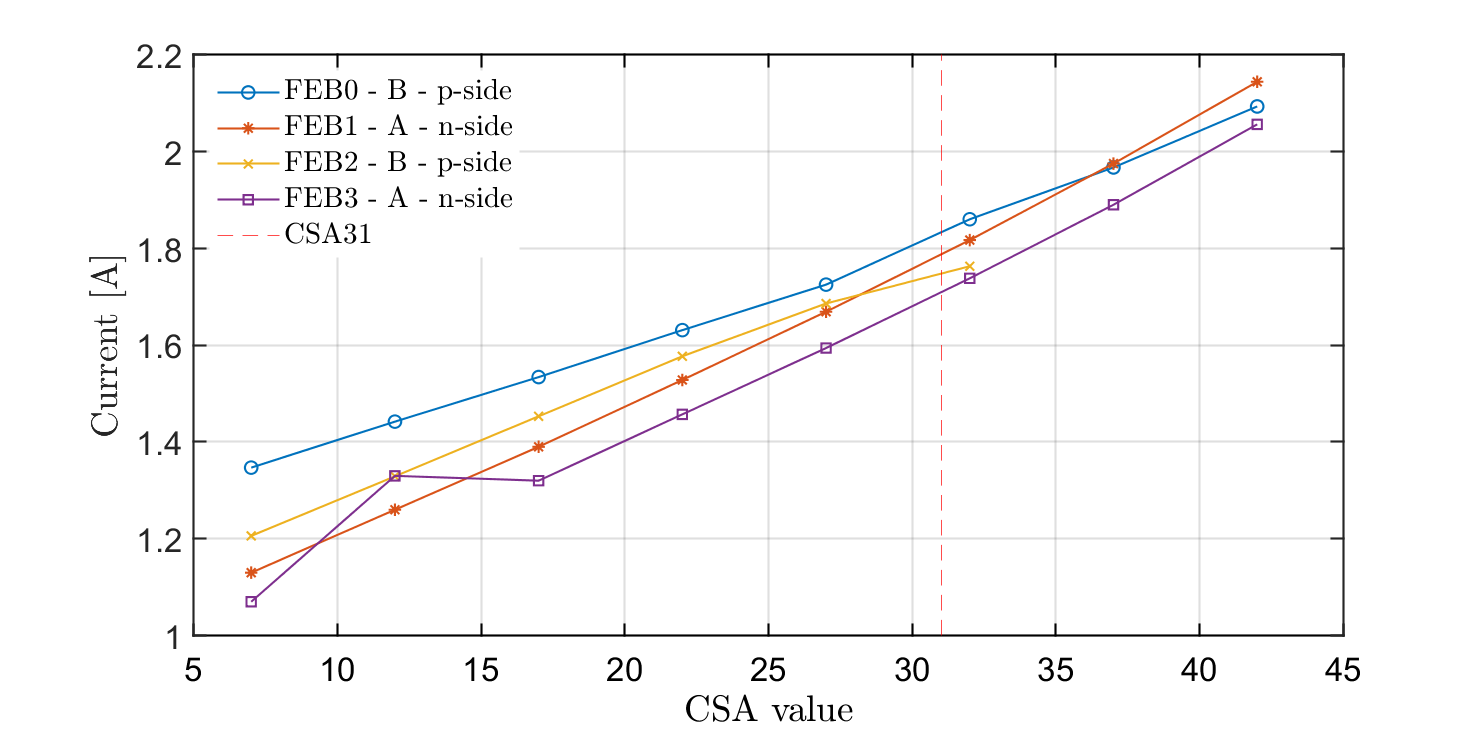
\includegraphics[width=0.9\columnwidth]{Chapter6/DCS/images/U3L1CSABIAS.png}
\caption{CSA scan of the unit 3 ladder 0}
\label{U3L1CSABIAS}
\end{figure}


\begin{figure}[h!]
\centering
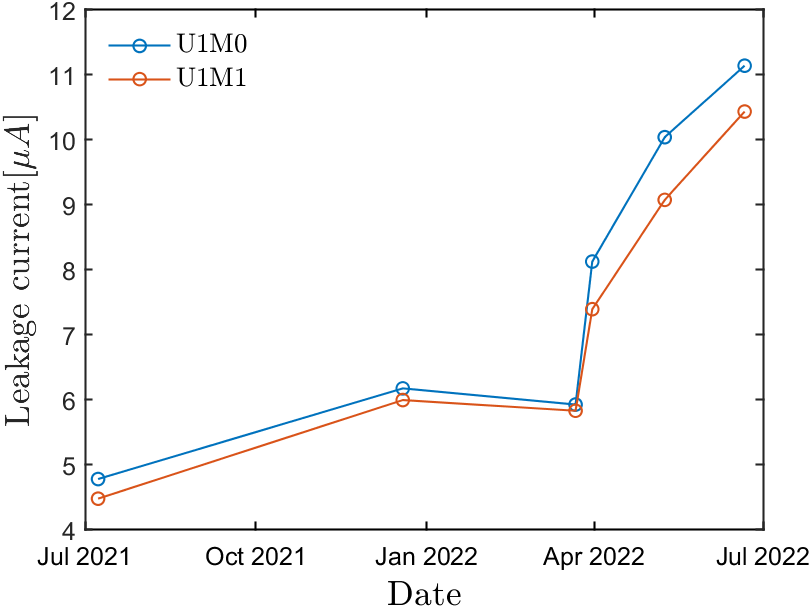
\includegraphics[width=0.45\columnwidth]{Chapter6/DCS/images/sensors/U1_leakage.png}
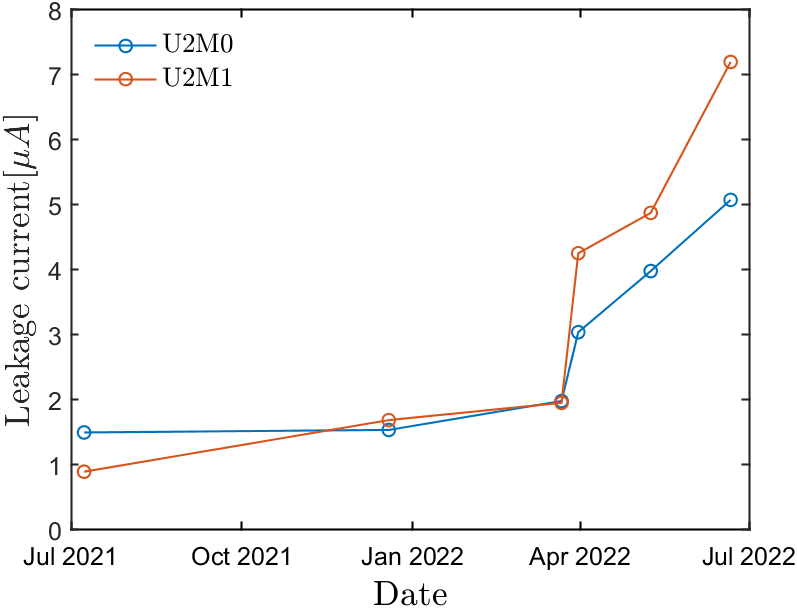
\includegraphics[width=0.45\columnwidth]{Chapter6/DCS/images/sensors/U2_leakage.png}
\caption{Leakage current evolution during the mSTS operation - Unit 1 and unit 2}
\label{leakage_current_u1u2}
\end{figure}

\begin{figure}[h!]
\centering
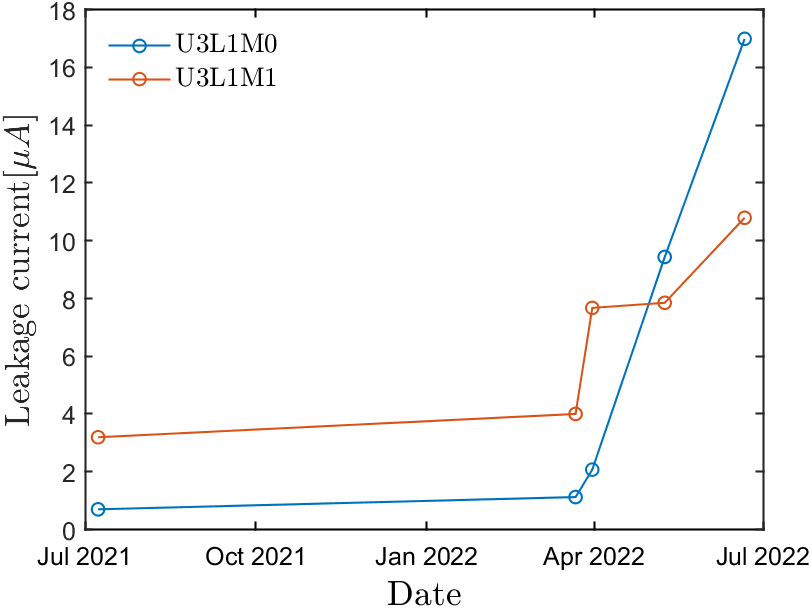
\includegraphics[width=0.55\columnwidth]{Chapter6/DCS/images/sensors/U3L1_leakage.png}
\caption{Leakage current evolution during the mSTS operation - Unit 3 ladder 1}
\label{leakage_current_u3l1}
\end{figure}





\begin{figure}[h!]
\centering
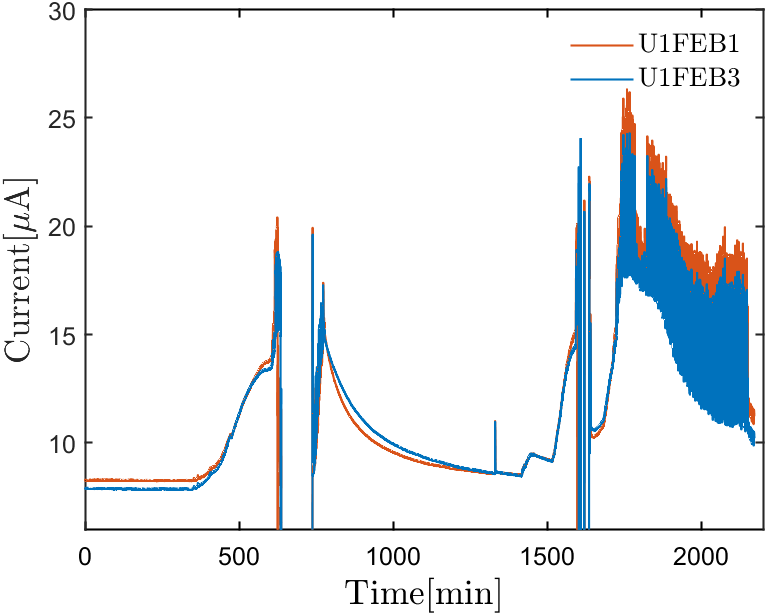
\includegraphics[width=0.45\columnwidth]{Chapter6/DCS/images/uranium/U1.png}
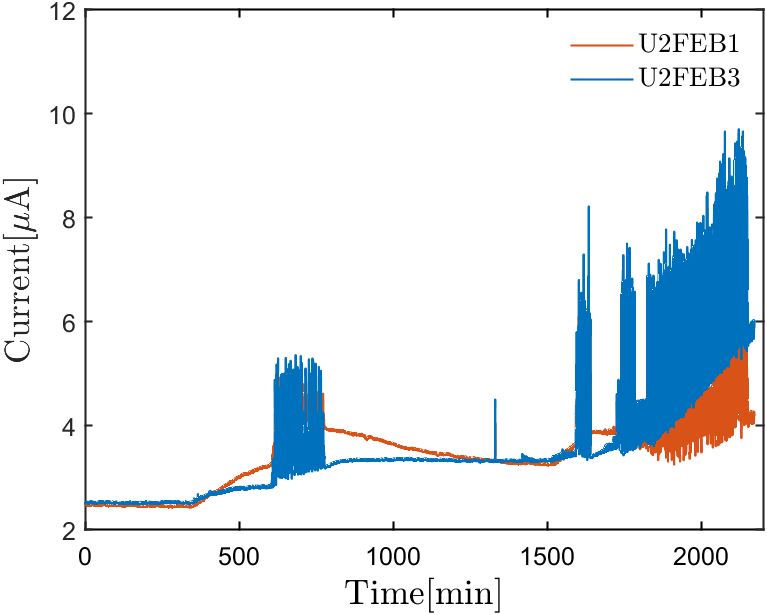
\includegraphics[width=0.45\columnwidth]{Chapter6/DCS/images/uranium/U2.png}
\caption{Unit 1 and unit 2 silicon sensors current}
\label{fig_U1U2}
\end{figure}

\begin{figure}[h!]
\centering
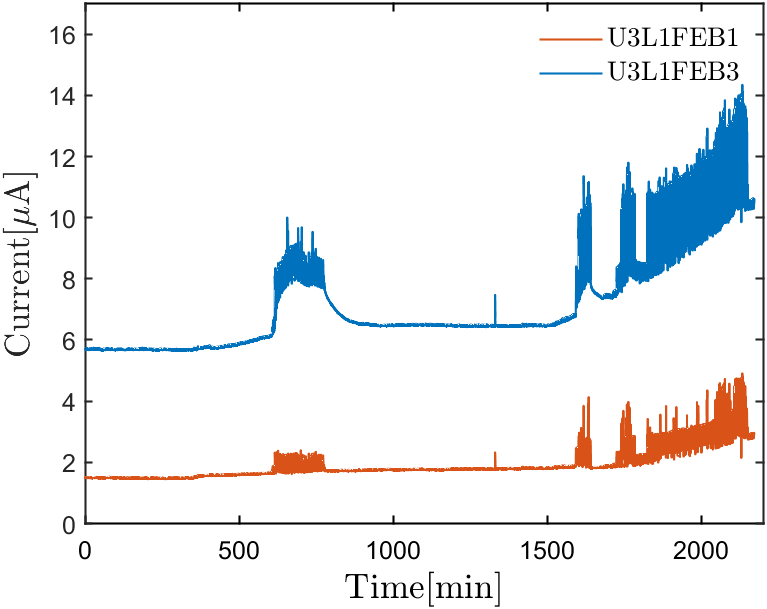
\includegraphics[width=0.55\columnwidth]{Chapter6/DCS/images/uranium/U3L1.png}
\caption{Unit 3 Ladder 1 silicon sensors current}
\label{fig_U3L1}
\end{figure}
%\chapter{IV curves}
%\label{IV}

\begin{figure}[h!]
\centering
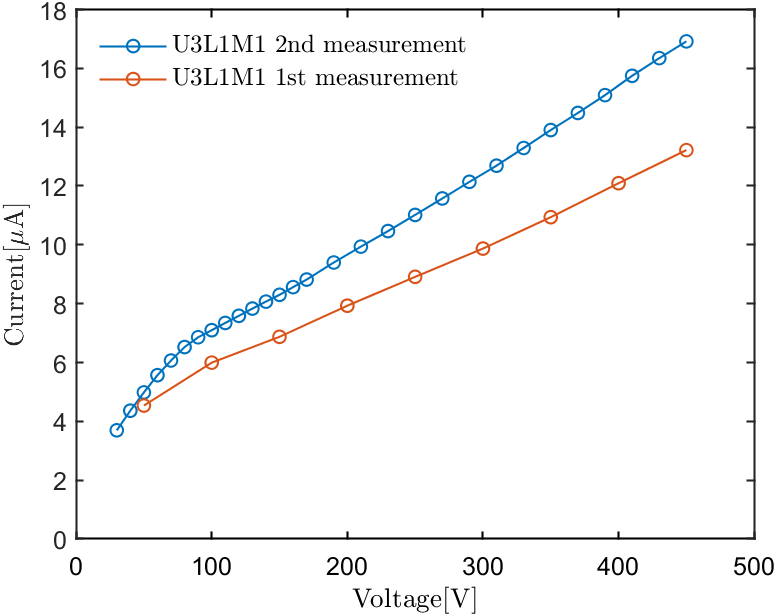
\includegraphics[width=0.47\columnwidth]{Chapter6/DCS/images/IV/U3L1FEB3.png}
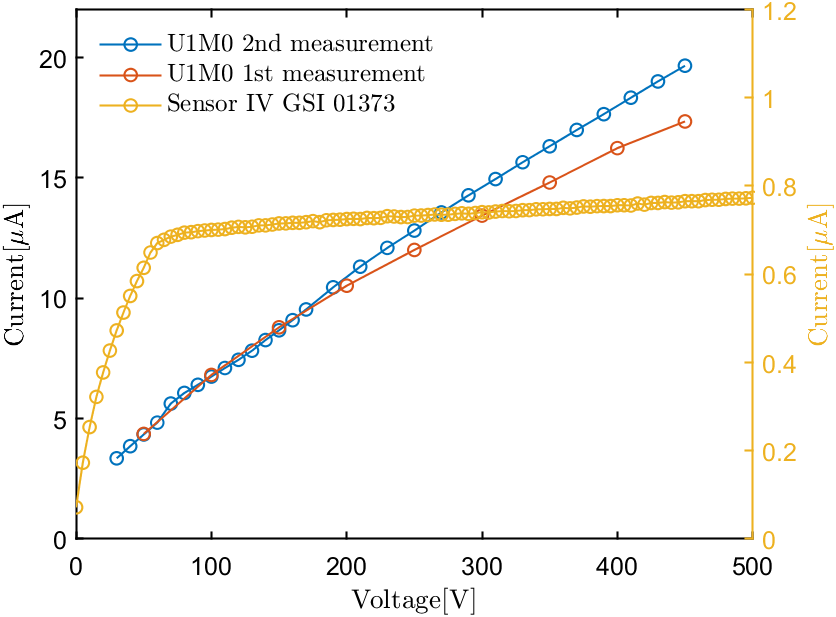
\includegraphics[width=0.49\columnwidth]{Chapter6/DCS/images/IV/U1FEB1.png}
\caption{IV curves for two modules from different units}
\label{fig_U1FEB1}
\end{figure}
